\documentclass[10pt,letterpaper]{article}
\usepackage[margin=1in]{geometry}
%\usepackage{natbib}
\usepackage{multicol}
\usepackage{graphicx}
\pagenumbering{gobble}
\usepackage{color}

\newcommand{\ea}[1]{{\color{blue}  #1}}

\title{\vspace{-2.5cm}A generative model for urban firm networks}
\author{J. Raimbault$^{1,2,3}$, N. Zdanowska$^{1,3}$ and E. Arcaute$^1$\\\medskip\small
$^{1}$ Centre for Advanced Spatial Analysis, UCL; $^{2}$ UPS CNRS 3611 ISC-PIF; $^{3}$ UMR CNRS 8504 G{\'e}ographie-cit{\'e}s
}
\date{}

\begin{document}

\maketitle

%\begin{abstract}
%    We introduce a generative network model for urban networks of interactions between firms. The growth of the network is simulated by adding new firm ownership links randomly, with probabilities determined by several factors, namely the economic size of origin and destination urban areas, industrial sector proximity, the strength of previous links, and geographical and socio-cultural distance. Simulation on synthetic systems of cities unveil phase transitions when changing interaction distance, and non-trivial patterns in model behavior. Future work include the calibration of the model on real company links for Europe.
%\end{abstract}

\vspace{-0.5cm}

The emergence of a global network of cities, defined by interactions between firms, is a salient feature of recent globalization processes \cite{taylor2001specification}. Understanding the drivers for growth for such a network, can be used to foster innovation through policies for local economic clusters \cite{turkina2016structure}, development of strategic industries for global insertion of regions \cite{dawley2019creating}, cities \cite{gluckler2016relational} and countries \cite{martinus2019brokerage}. Linkages are characterized by interactions of different nature and determined by economic, socio-cultural, or geopolitical proximity \cite{martinus2018global}.


This paper focuses on economic relations between urban areas defined by ownership links of firms. Since transnational firms structure is one of the determinant of the global economic space, it is one of the proxies to unveil geographical structures \cite{2019arXiv191014652Z}. 
This work introduces a generative network model to simulate the growth of such linkages at urban areas scale within the evolutionary systems of cities framework \cite{pumain2018evolutionary}. We combine multiple factors which influence link formation, as economic intensity of origin and destination of urban areas, industrial sector proximity, the strength of previous links, and geographical and socio-cultural distance. The model allows thus to compare the effect of different factors on the final network structure, and to extrapolate their actual effect when calibrated on real data.


Formally, the model creates links between cities which are characterized by their economic size $E_i$ (GDP) and economic structure $S_{ik}$ in terms of activity sectors (probability distribution of firms within $K$ sectors). Starting with an existing network with no links, the model iteratively adds links, following a probability given by a generalized Cobb-Douglas function \cite{vilcu2011geometric} as 
\[
p_{ij} \propto \left(\frac{E_{i}}{E}\right)^{\gamma_F} \cdot \left(\frac{E_{j}}{E}\right)^{\gamma_T} \cdot \left(\frac{w_{ij}}{W}\right)^{\gamma_W} \cdot s\left(S_{ik},S_{jk}\right)^{\gamma_S} \cdot \exp \left(- \gamma_G \cdot d_{ij}\right) \cdot \exp \left(- \gamma_D \cdot g_{ij}\right)
\]
where $E  =  \sum_k E_k$, $W  = \sum_{i,j} w_{ij}$ weights of previous links, $s(S_{ik},S_{jk})$ is similarity function between activity sectors $S_{ik}$ and $S_{jk}$, $d_{ij}$ euclidian distance, and $g_{ij}$ a socio-cultural distance. In the case of an already existing link between two areas, the weight of the latter is incremented by one. The model is stopped either when a final time is reached or when a given number of links have been added. This formulation can be considered both as an economic utility and a generalization of spatial interaction models. The model parameters are the Cobb-Douglas weights $\gamma_F,\gamma_T,\gamma_W,\gamma_s$ and distance decay parameters $\gamma_G,\gamma_D$. The model also includes path-dependency by integrating the influence of previous links. Therefore it can not be reduced to a simple statistical model. Finally, the role of space introduces even further complexity, yielding a generative model, which has to be simulated.

We consider several macroscopic indicators to quantify the generated network. Firstly, geographical structures are captured by (i) internationalisation (modularity of countries in the network); (ii) metropolisation (correlation between weighted degree and city size); (iii) regionalisation (correlation between length and flow of links, stratified by size of extremities); and (iv) Specialisation (correlation between sector proximity and flow of links, stratified by size of extremities). We also consider several network indicators as Louvain modularity, community sizes, degree and link weight distributions (described by their average, hierarchy, and entropy), and correlations between degree and city size, and between link weight and distance.

The model is implemented in NetLogo and integrated into the OpenMOLE platform for model exploration to distribute the computation on high performance infrastructures. We build the model on a synthetic system of cities, at the scale of a continent with properties similar to Europe: (i) 700 cities with an empirical power-law from the Global Human Settlements database for economic sizes; (ii) clustered into 30 countries; (iii) with synthetic distribution of sectors following log-normal distributions adjusted in a way that large cities have more high-value activities and are more diverse. The network is generated from an empty initial network until reaching $t_f=1500$. A first numerical experiment of one-factor sampling on all Cobb-Douglas parameters and 100 stochastic repetitions confirms a good statistical convergence (average Sharpe ratios for indicators all larger than 5). The model behaviour is then studied with a grid sampling for parameters and 20 repetitions (the computations run on the European Grid Infrastructure, and are equivalent to 2.5 years of CPU time).

We show in Fig. 1 examples of generated networks, with very contrasted patterns obtained with different spatial interaction ranges. This behavior is confirmed when plotting the internationalization index against the distance, which shows an exponential decay. Similarly, the correlation between city weighted degree and city size exhibit a behaviour that can be interpreted as a phase transition between local and global networks. Other indicators exhibit non-trivial patterns. For example, when considering average community size of the final network, we obtain a maximal integration in term of communities at an intermediate value of the gravity decay, what can be interpreted as the emergence of a regional regime. The size of communities is largely influenced by the value of the elasticities for the similarity function and the ratio of the economic output of the area. Altogether, these experiments reveal a complex interplay between processes and how the model produces diverse stylized facts.

As a matter of validation, the model is implemented for real data for Europe joining Functional Urban Areas with the Global Human Settlement Database for cities and their characteristics, with the AMADEUS database produced by the Bureau Van Dijk on ownership links between firms in Europe between 2010 and 2018 at postcode level in all types of sectors. Calibration is done using a genetic NSGA2 algorithm, finding the parameter values giving network trajectories closest to reality. First results show in particular a role of the path-dependency parameter confirming the relevance of this complex generative model. Further work is needed to get more conclusions from this experiment but we already show the feasibility of model calibration on real data.

Several scenarios are considered taking into consideration the current and future economic challenges, such as those given by Brexit. This way, the model may be applied in future work to concrete policy questions.


\begin{figure}
\vspace{-2cm}
\begin{center}
    \begin{minipage}[c]{0.25\textwidth}
        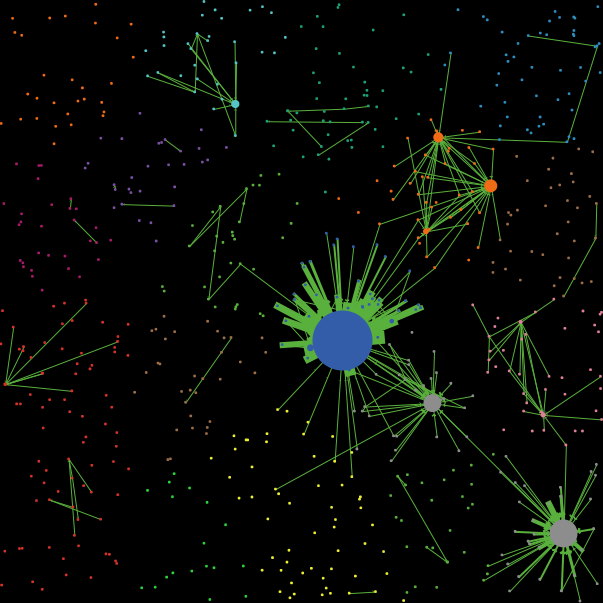
\includegraphics[width=\textwidth]{figures/ex_alleq-lowgravity_seed-12102_t1500.png}\\
        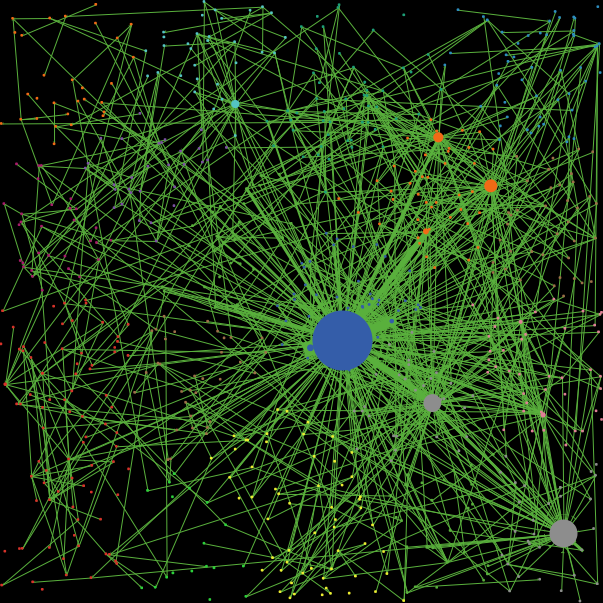
\includegraphics[width=\textwidth]{figures/ex_alleq-highgravity_seed-12102_t1500.png}
    \end{minipage}
    \begin{minipage}[c]{0.6\linewidth}
     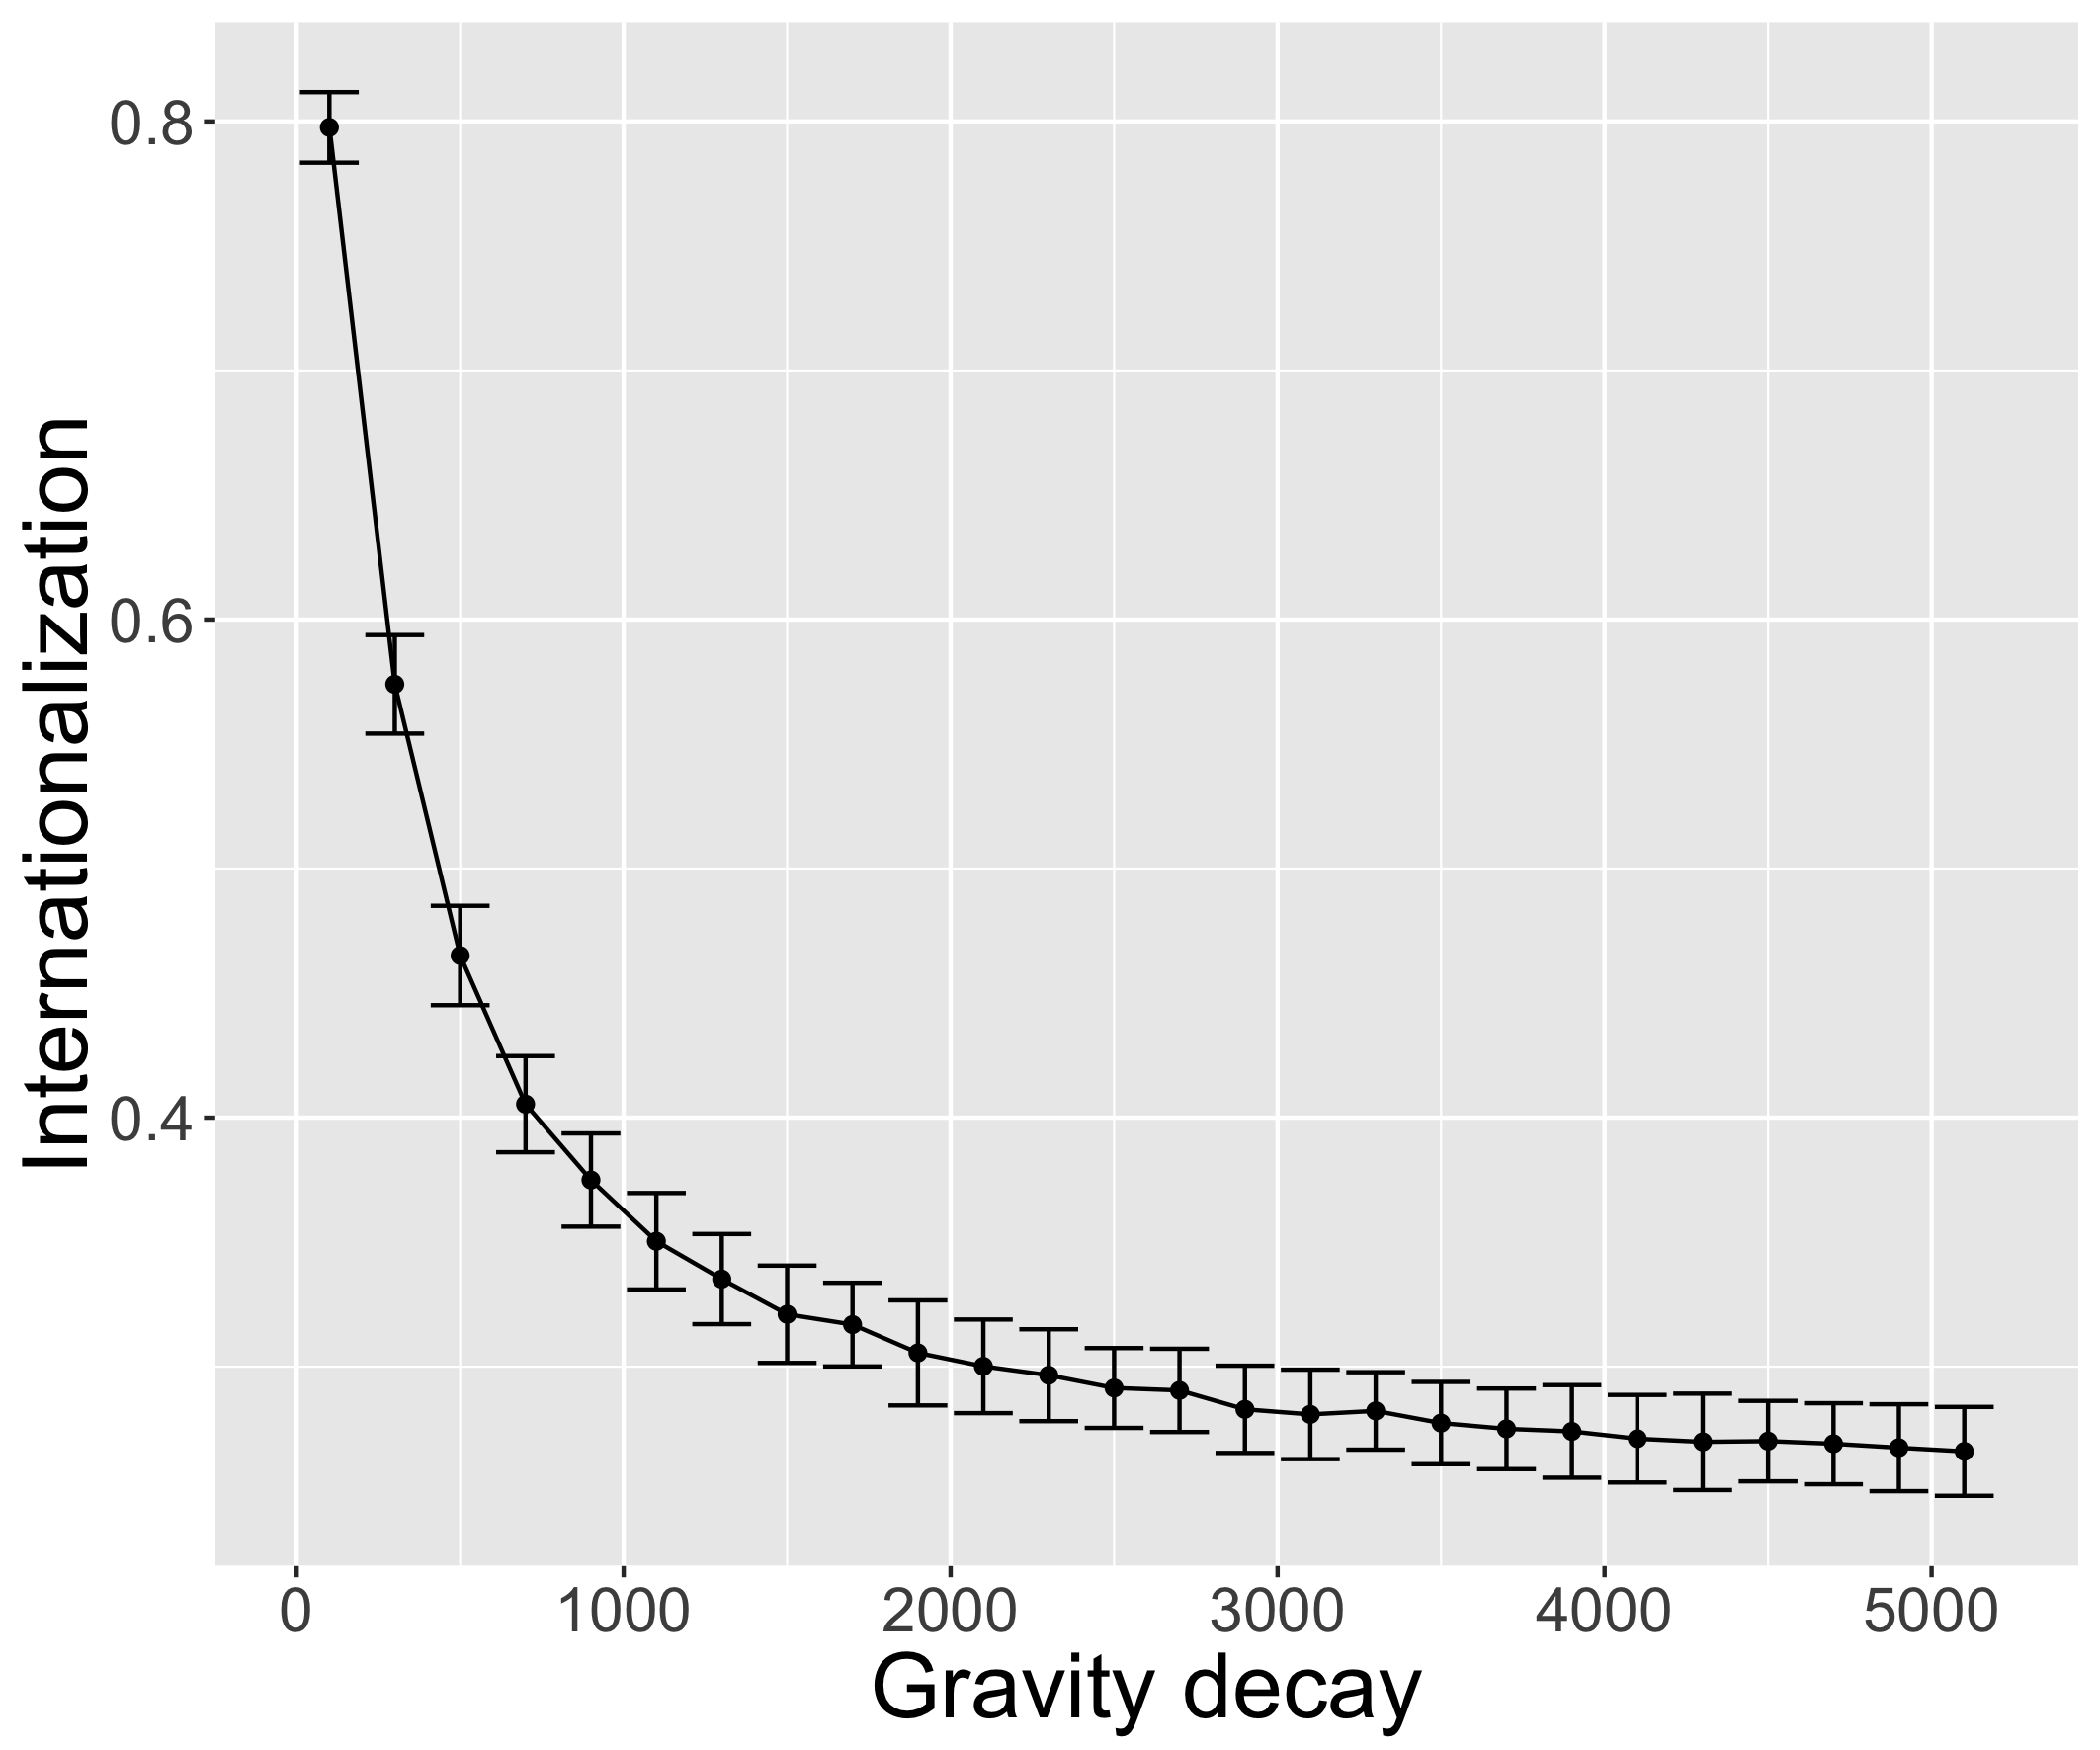
\includegraphics[width=0.48\textwidth]{figures/internationalization-gravityDecay_errorbars.png}
    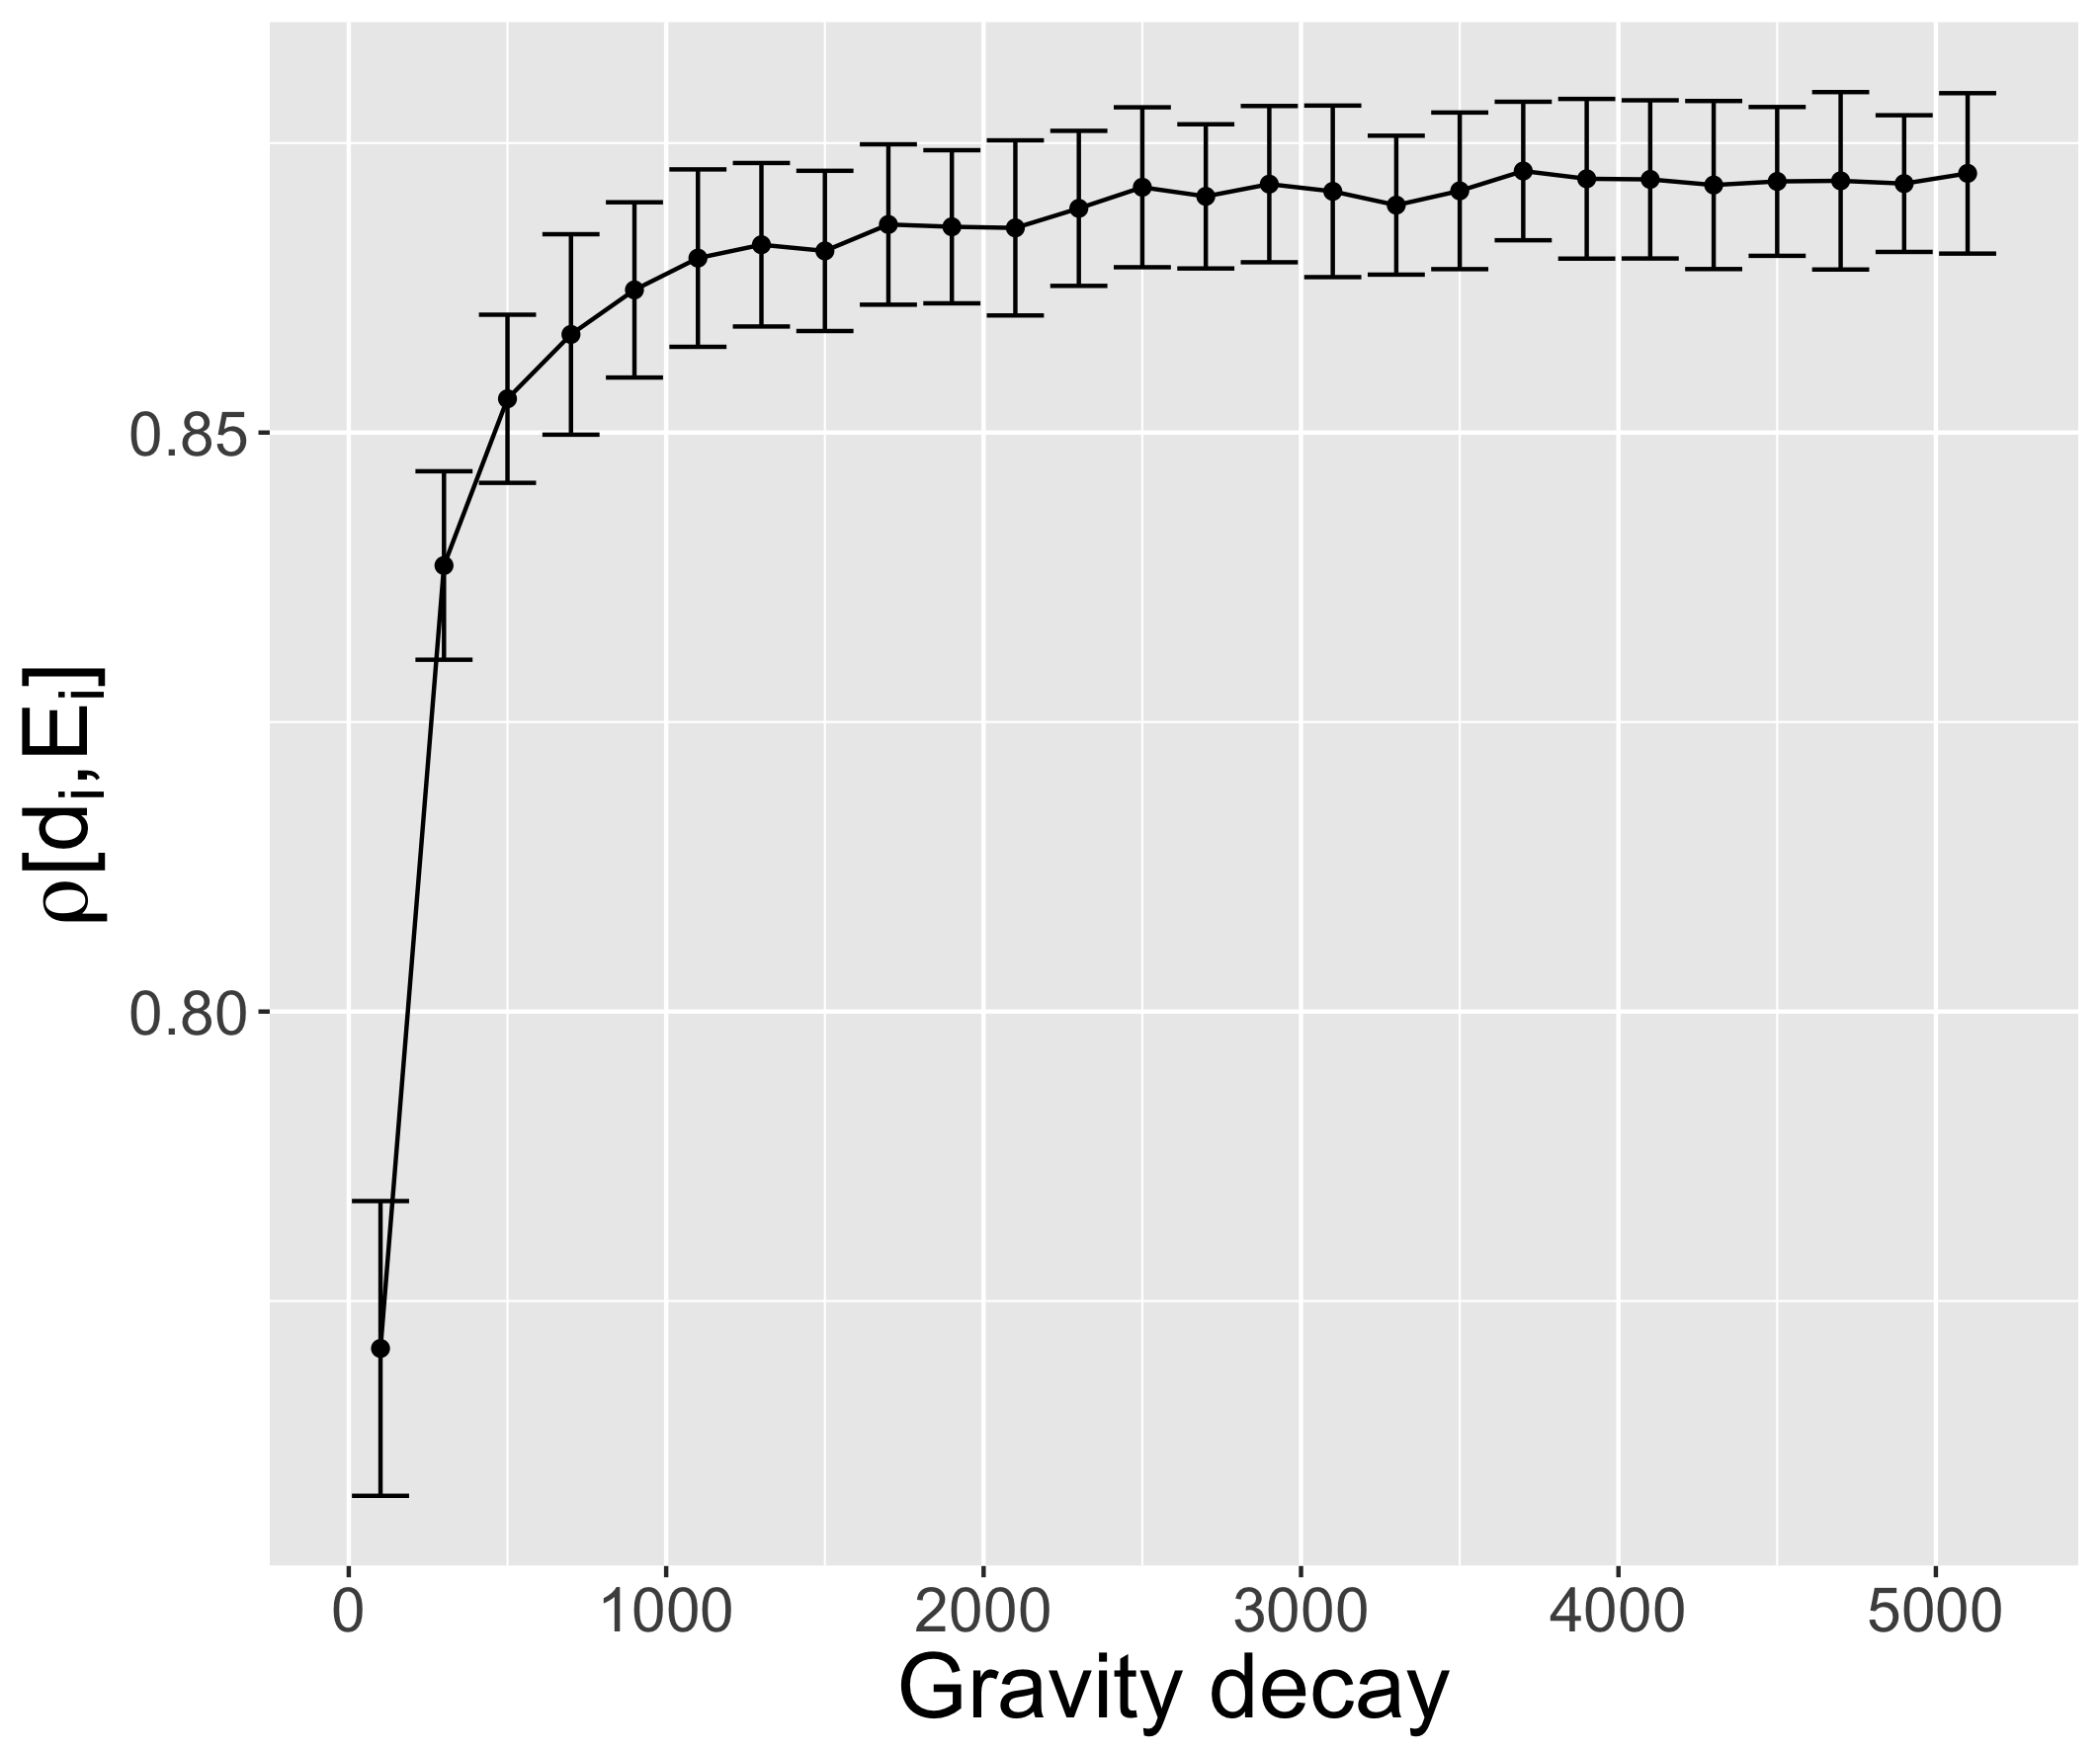
\includegraphics[width=0.48\textwidth]{figures/rhoDegreeSize-gravityDecay_errorbars.png}\\
    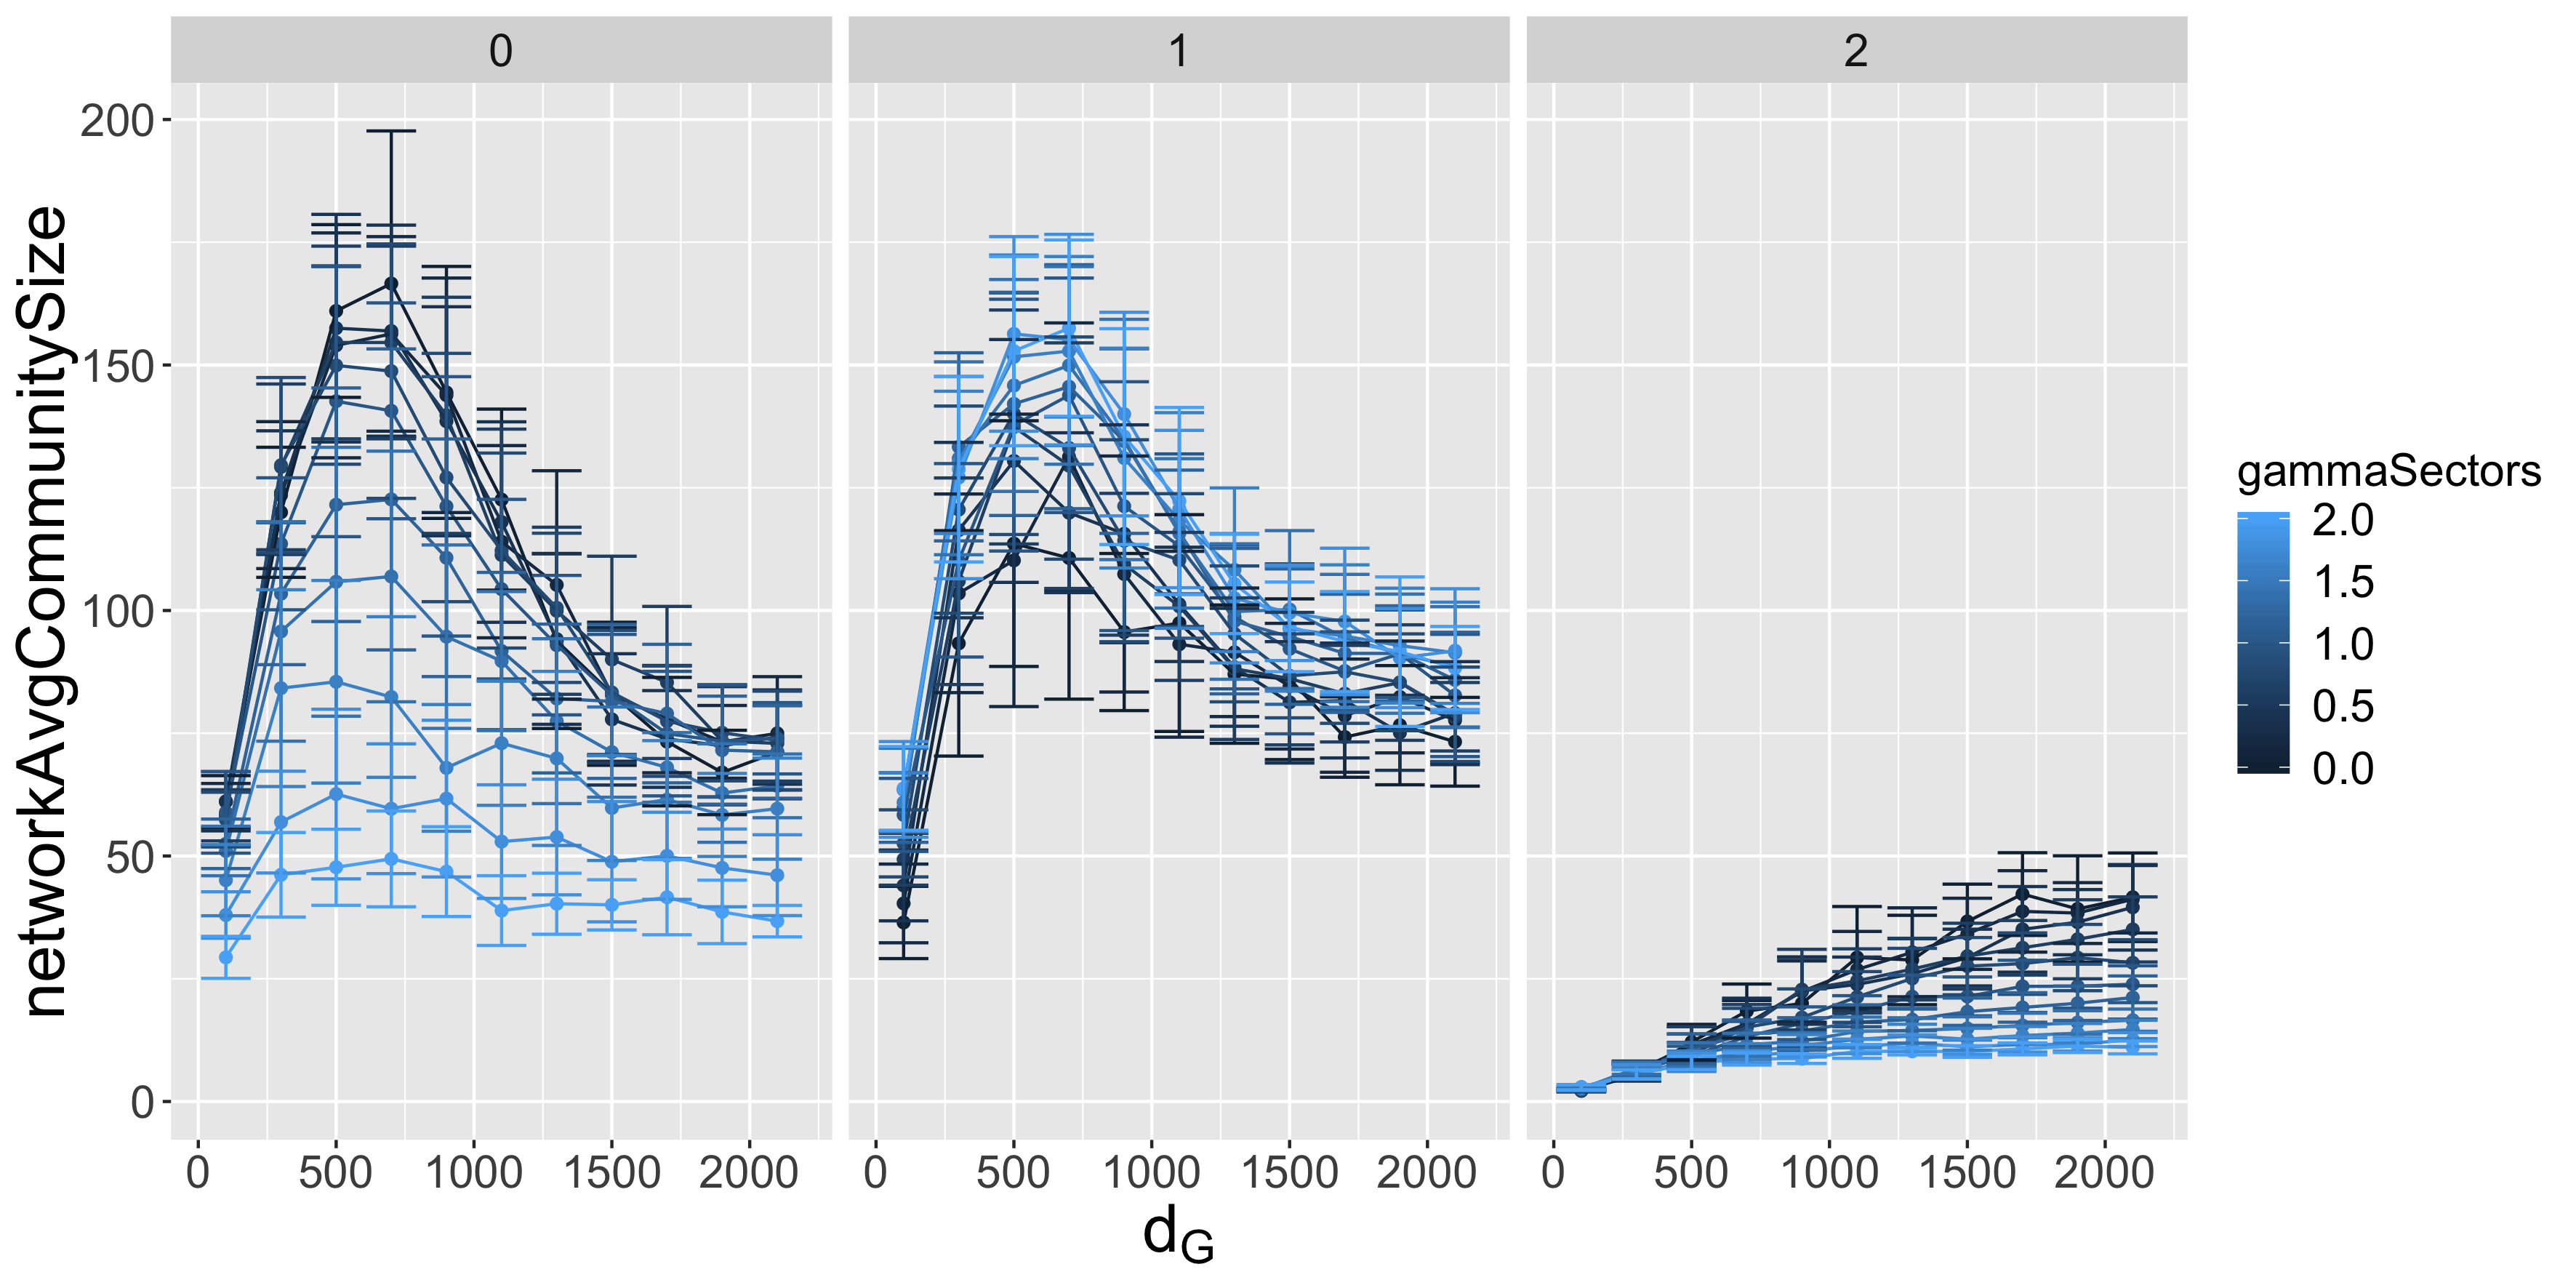
\includegraphics[width=\textwidth]{figures/networkAvgCommunitySize_countryGravityDecay2100_gammaDestination0_facetwrapgammaOrigin_colorgammaSectors.png}
    \end{minipage}
    \end{center}
    \vspace{-0.5cm}
    \caption{\footnotesize\textbf{(Left column)} Example of simulated networks for a synthetic system of cities, with low gravity range (top) and high gravity range (bottom); \textbf{(Top right)} Internationalization and correlation between size and degree as a function of decay parameter; \textbf{(Bottom right)} Average network community size as a function of decay parameter, for varying influence of sectors ($\gamma_S$ in color) and of origin ($\gamma_F$ in columns).}
\end{figure}


\footnotesize


\begin{multicols}{2}

\bibliographystyle{unsrt}
\bibliography{biblio}

\end{multicols}

\end{document}